\section{Numerical Examples}

\sectioncover

\subsection{Three-point bending}

\begin{frame}
  \begin{columns}[T]
    \begin{column}{0.6\textwidth}
      \vspace{-1em}
      \begin{figure}
        \centering
        \begin{subfigure}{0.32\linewidth}
          \centering
          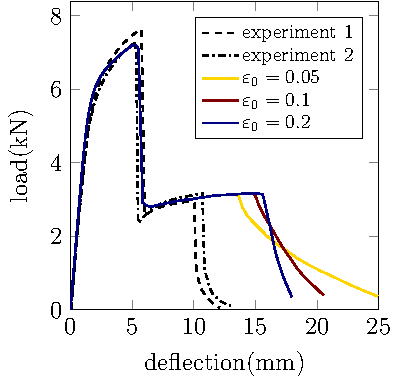
\includegraphics[width=0.8\textwidth]{examples/figures/Chapter5-3pb-load_deflection-constant_beta}
        \end{subfigure}
        \begin{subfigure}{0.32\linewidth}
          \centering
          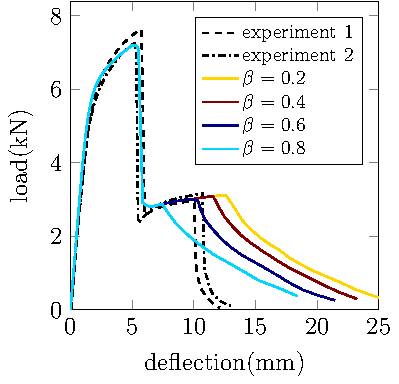
\includegraphics[width=0.8\textwidth]{examples/figures/Chapter5-3pb-load_deflection-constant_e0}
        \end{subfigure}
        \begin{subfigure}{0.32\linewidth}
          \centering
          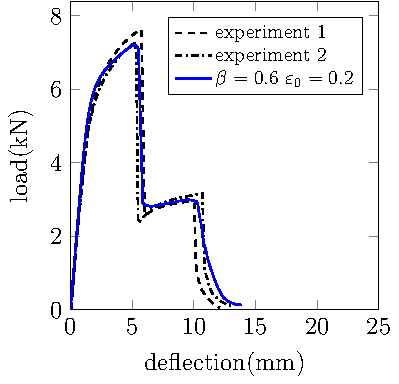
\includegraphics[width=0.8\textwidth]{examples/figures/Chapter5-3pb-load_deflection_tuned}
        \end{subfigure}
        
        \vspace{0.5em}
        
        \begin{subfigure}{0.45\textwidth}
          \centering
          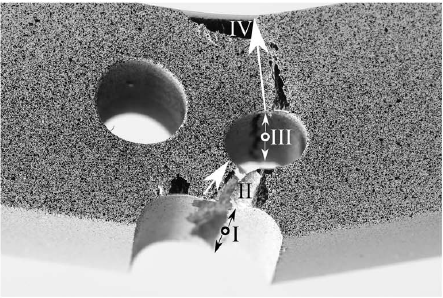
\includegraphics[width=0.7\textwidth,scale=0.5]{examples/figures/1234}
        \end{subfigure}
        \only<1>{
          \begin{subfigure}{0.45\textwidth}
            \centering
            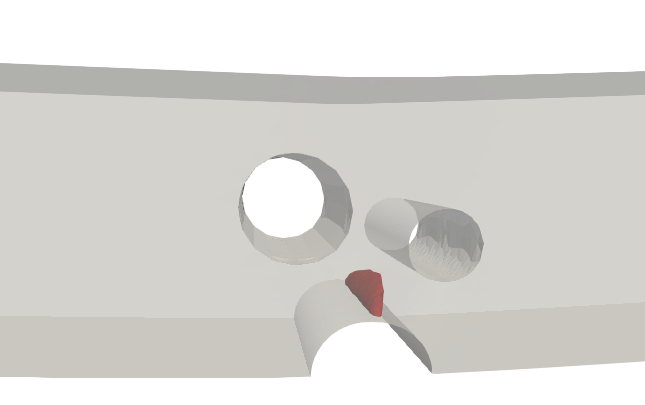
\includegraphics[width=0.7\textwidth]{examples/figures/I}
          \end{subfigure}
        }
        \only<2>{
          \begin{subfigure}{0.45\textwidth}
            \centering
            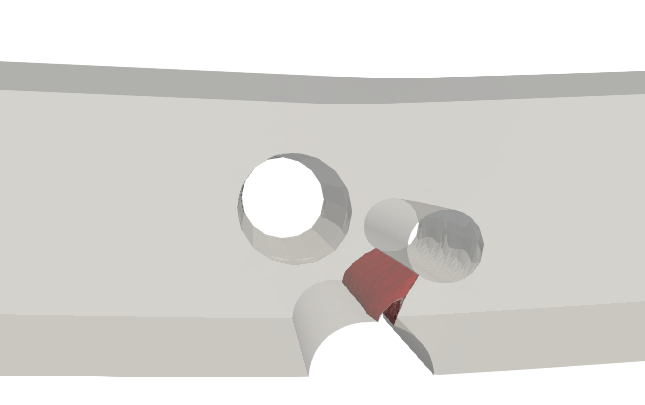
\includegraphics[width=0.7\textwidth]{examples/figures/II}
          \end{subfigure}
        }
        \only<3>{
          \begin{subfigure}{0.45\textwidth}
            \centering
            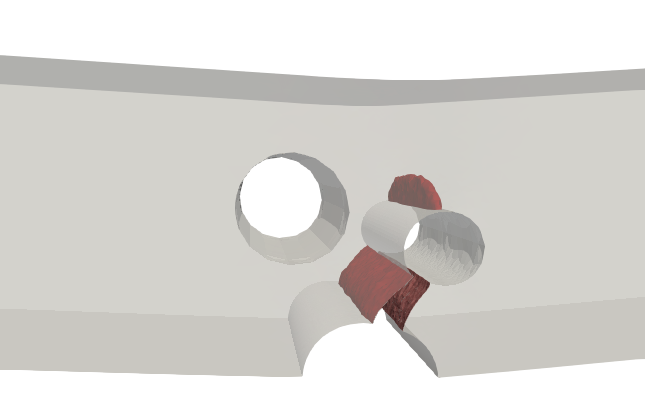
\includegraphics[width=0.7\textwidth]{examples/figures/III}
          \end{subfigure}
        }
        \only<4>{
          \begin{subfigure}{0.45\textwidth}
            \centering
            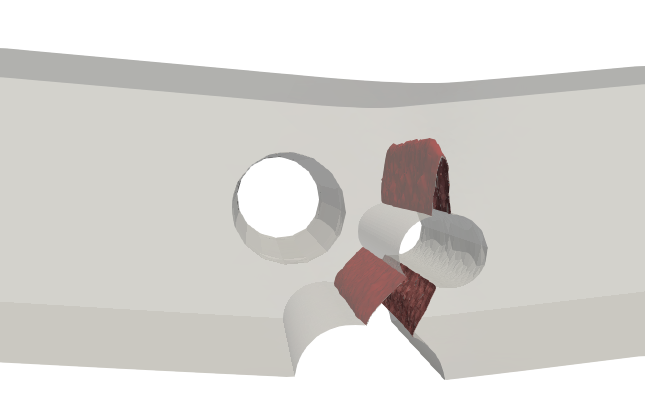
\includegraphics[width=0.7\textwidth]{examples/figures/IV}
          \end{subfigure}
        }
        
        \vspace{0.5em}
        
        \begin{subfigure}[b]{0.45\textwidth}
          \centering
          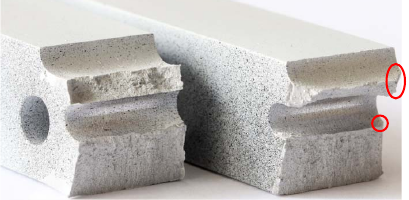
\includegraphics[width=0.9\textwidth,scale=0.5]{examples/figures/split_experiment}
        \end{subfigure}
        \begin{subfigure}[b]{0.45\textwidth}
          \centering
          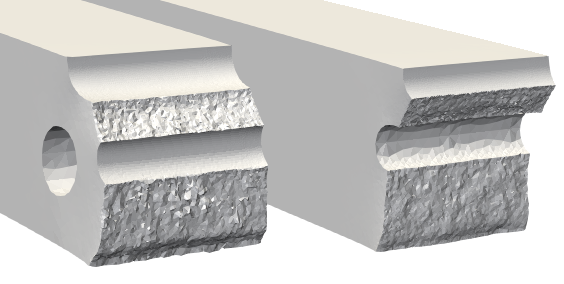
\includegraphics[width=0.9\textwidth,scale=0.5]{examples/figures/split}
        \end{subfigure}
      \end{figure}
    \end{column}
    \begin{column}{0.4\textwidth}
      \begin{itemize}
        \item A \textcolor{peggyblue}{three-point bending} experiment is simulated.
        \item The \textcolor{peggyblue}{aluminum} specimen is modeled as a \textcolor{peggyblue}{compressible Neo-Hookean} material, with \textcolor{peggyblue}{linear hardening}, \textcolor{peggyblue}{$\tqf = 1$}.
        \item \textcolor{peggyblue}{Coalescence dissipation} is included. The effects of $\beta$ and $\varepsilon_0$ are investigated in a 2D setting.
        \item Parameters are calibrated based on a \textcolor{peggyblue}{tensile tension test}.
        \item ``Shear lips'' are not captured by numerical simulations.
        \item Crack paths and load deflection curves have \textcolor{peggyblue}{excellent agreement} with the experiment.
      \end{itemize}
    \end{column}
  \end{columns}
\end{frame}

\subsection{The Sandia Fracture Challenge}

\begin{frame}
  \vspace{-1.5em}
  \begin{columns}[T]
    \begin{column}{0.6\textwidth}
      \vspace{-1em}
      \begin{figure}
        \centering
        \begin{subfigure}{0.95\linewidth}
          \centering
          \begin{tikzpicture}
            \node[inner sep=0] (mesh) at (0,0) {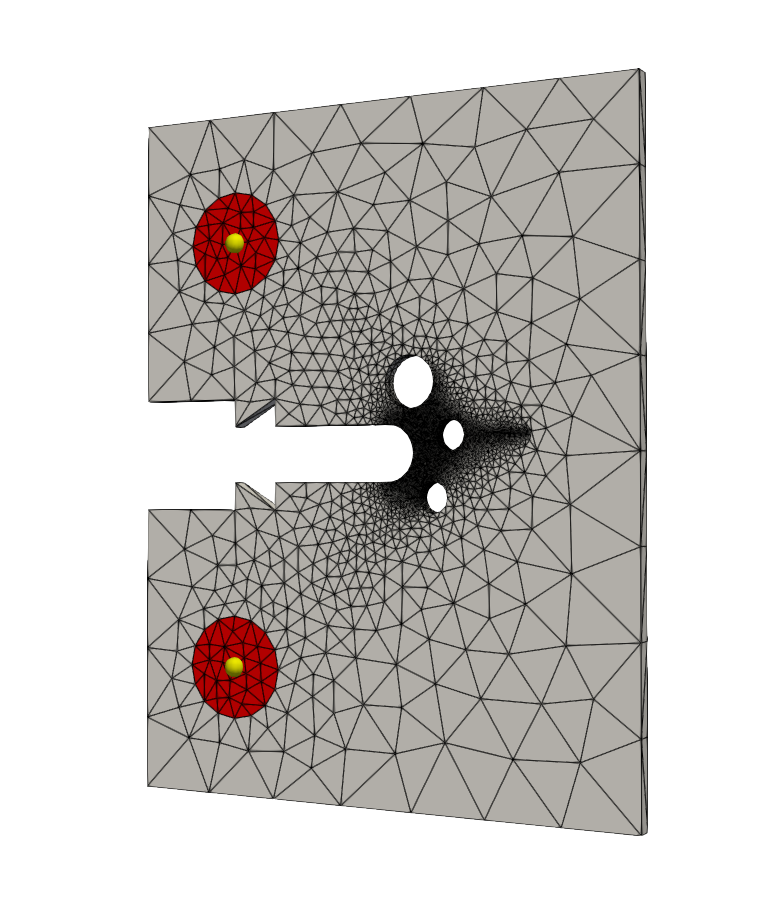
\includegraphics[width=0.3\textwidth,scale=0.5]{examples/figures/mesh}};
            \coordinate (box_sw) at (-0.15, -0.4);
            \coordinate (box_nw) at (-0.15, 0.48);
            \coordinate (box_ne) at (0.5, 0.55);
            \coordinate (box_se) at (0.5, -0.43);
            
            \draw [blue] (box_sw) -- (box_nw);
            \draw [blue] (box_nw) -- (box_ne);
            \draw [blue] (box_ne) -- (box_se);
            \draw [blue] (box_se) -- (box_sw);
            
            \node[inner sep=0] (meshzoom) at (3,0) {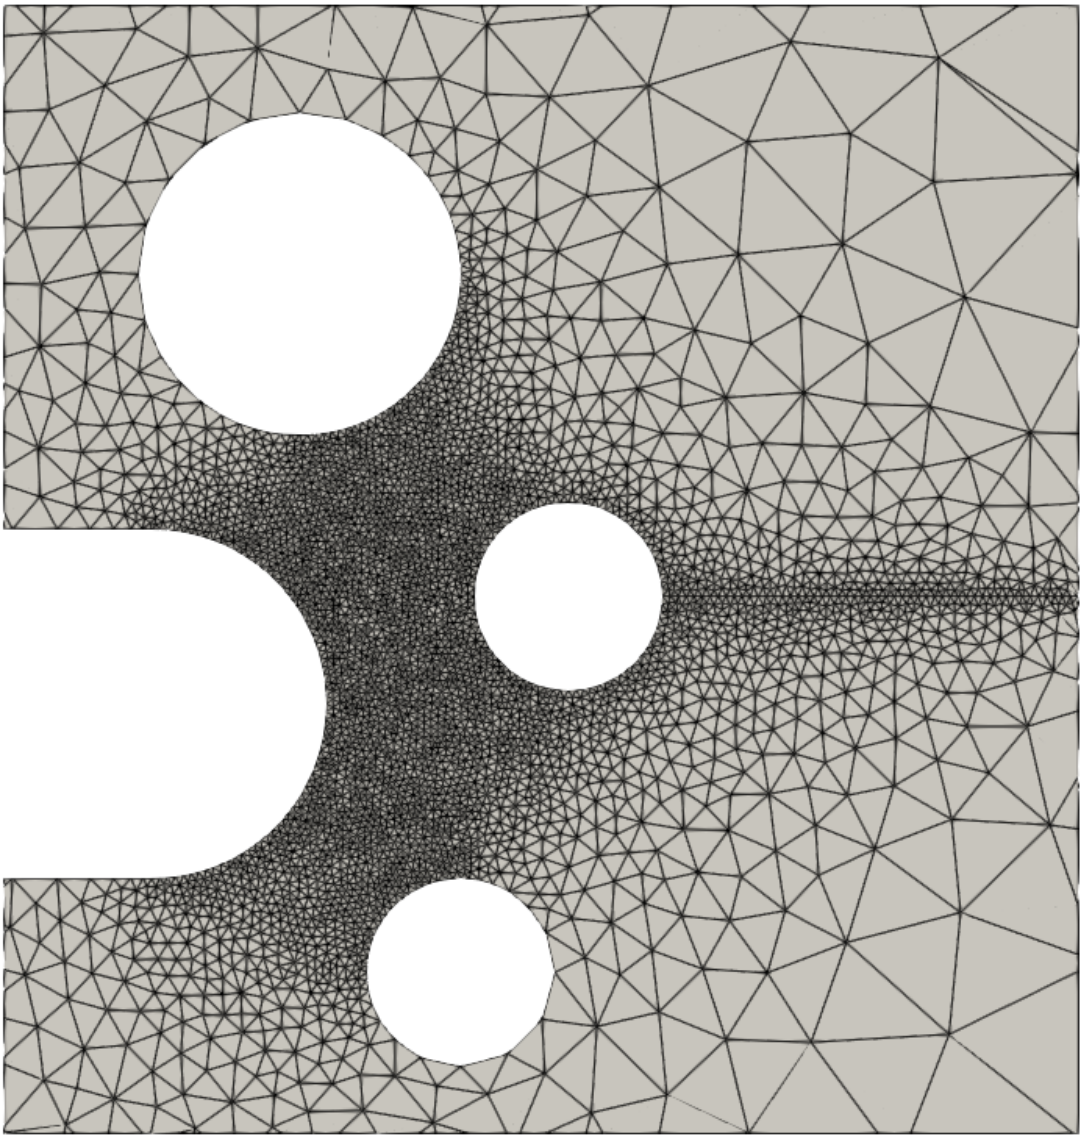
\includegraphics[width=0.3\textwidth,scale=0.5]{examples/figures/meshzoom}};
            \node (boxzoom) at (meshzoom.south west) [draw,blue,thick,minimum width=0.3\textwidth,minimum height=72,anchor=south west] {};
            
            \draw (box_ne) -- (boxzoom.north west);
            \draw (box_se) -- (boxzoom.south west);
            
            \node (A) at (-0.45,0.85) [yellow] {\textbf{A}};
            \node (B) at (-0.45,-0.85) [yellow] {\textbf{B}};
          \end{tikzpicture}
        \end{subfigure}
        
        \begin{subfigure}{0.32\textwidth}
          \centering
          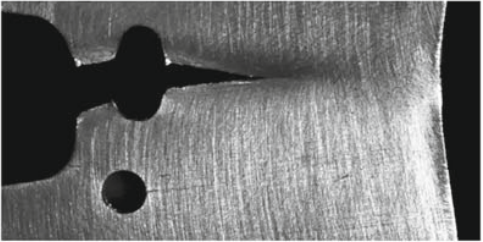
\includegraphics[width=\textwidth]{examples/figures/SFC_schematics}
        \end{subfigure}
        \begin{subfigure}{0.32\textwidth}
          \centering
          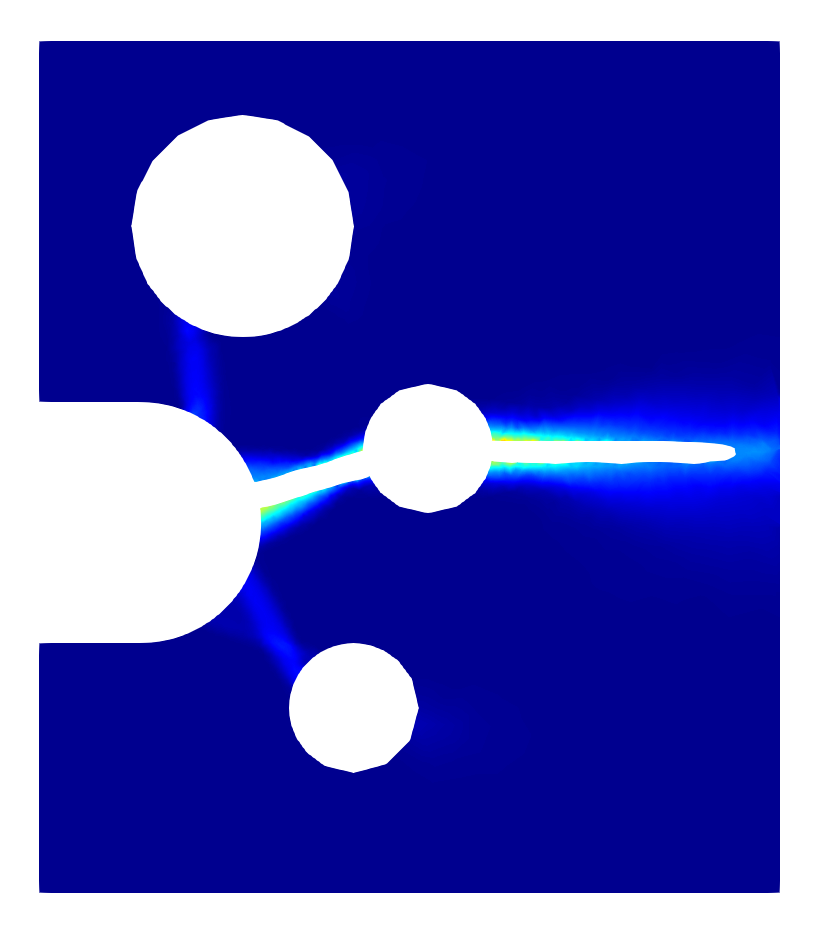
\includegraphics[width=0.55\textwidth]{examples/figures/W_pl_3}
        \end{subfigure}
        \begin{subfigure}{0.32\textwidth}
          \centering
          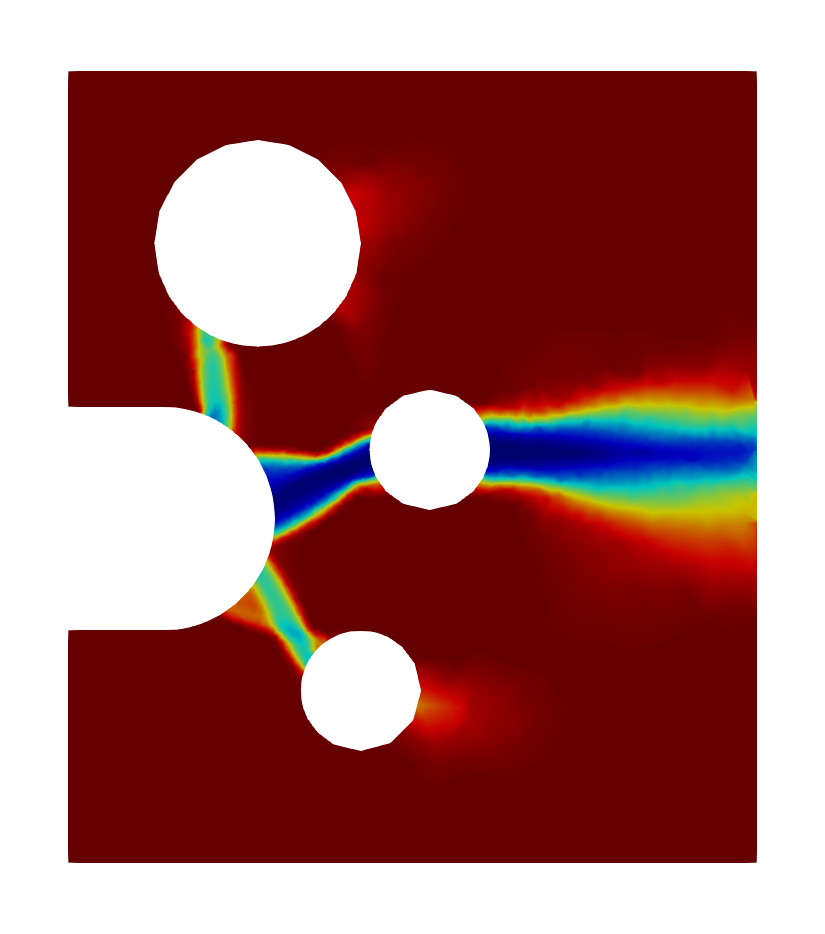
\includegraphics[width=0.62\textwidth]{examples/figures/M_3}
        \end{subfigure}
        
        \begin{subfigure}{0.95\textwidth}
          \begin{tikzpicture}
            \begin{axis}[
                cycle list name=exotic,
                width=\textwidth,
                height=0.4\textwidth,
                xmin=0,xmax=7,
                ymin=0,
                xlabel=displacement(\SI{}{\milli\meter}),ylabel=force(\SI{}{\kilo\newton}),
                scaled y ticks=false,
                xticklabel style={
                    /pgf/number format/fixed,
                    /pgf/number format/precision=2
                  },
                legend style={
                    at={(0.1,0.05)},
                    anchor=south west,
                    nodes={scale=0.6, transform shape},
                    fill=none,
                    draw=none,
                    cells={align=left}
                  },
                legend cell align={left},
                every axis plot/.append style={thick}
              ]
              \addplot +[mark=none,black,dashed] table[x expr=\thisrowno{0},y expr=\thisrowno{1}/1000,col sep=comma]{examples/data/experiment.csv};
              \addplot +[mark=none] table[x expr=\thisrowno{0},y expr=\thisrowno{1}/1000,col sep=comma]{examples/data/force_disp.csv};
              \addplot +[mark=none] table[x expr=\thisrowno{0},y expr=\thisrowno{1}/1000,col sep=comma]{examples/data/force_disp_lorenzis_1.csv};
              \addplot +[mark=none] table[x expr=\thisrowno{0},y expr=\thisrowno{1}/1000,col sep=comma]{examples/data/force_disp_lorenzis_2.csv};
              \legend{experiment,proposed E-P-D model,prediction with $m=1$ from Ambati et al.,prediction with $m=2$ from Ambati et al.}
            \end{axis}
          \end{tikzpicture}
        \end{subfigure}
      \end{figure}
    \end{column}
    \begin{column}{0.4\textwidth}
      \begin{itemize}
        \item A recent \textcolor{peggyblue}{Sandia Fracture Challenge}.
        \item Material properties are calibrated using provided \textcolor{peggyblue}{tensile tension test} data.
        \item Loading pins A and B are modeled as purely elastic materials with the same constants as the specimen.
        \item The predicted \textcolor{peggyblue}{force-displacement curve} is compared with the experimental data and predictions by other existing phase-field models of ductile fracture.
        \item The agreement between the experiment and our simulation is \textcolor{peggyblue}{remarkable}, both in terms of the crack path and the force-displacement curve.
      \end{itemize}
    \end{column}
  \end{columns}
\end{frame}

\subsection{Oxide spallation in high temperature heat exchangers}

\begin{frame}
  \vspace{-1.5em}
  \begin{columns}[T]
    \begin{column}{0.6\textwidth}
      \begin{figure}
        \centering
        \only<1-7>{
          \begin{subfigure}{0.3\textwidth}
            \centering
            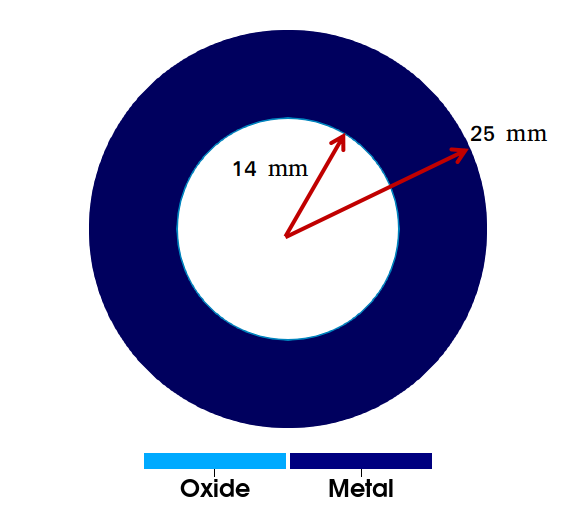
\includegraphics[width=\textwidth]{examples/figures/top_view}
          \end{subfigure}
          \begin{subfigure}{0.3\textwidth}
            \centering
            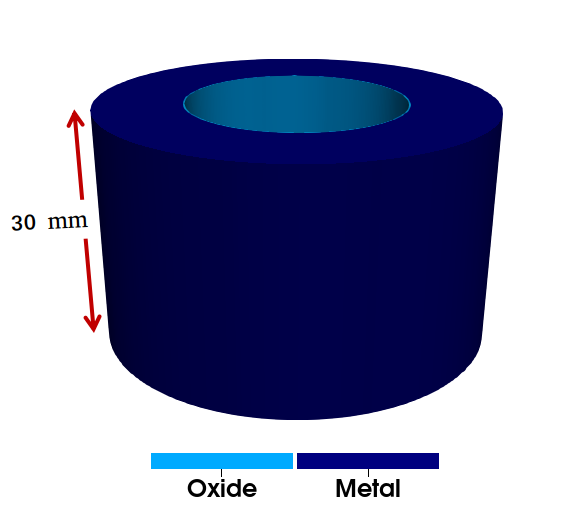
\includegraphics[width=\textwidth]{examples/figures/side_view}
          \end{subfigure}
          \begin{subfigure}{0.3\textwidth}
            \centering
            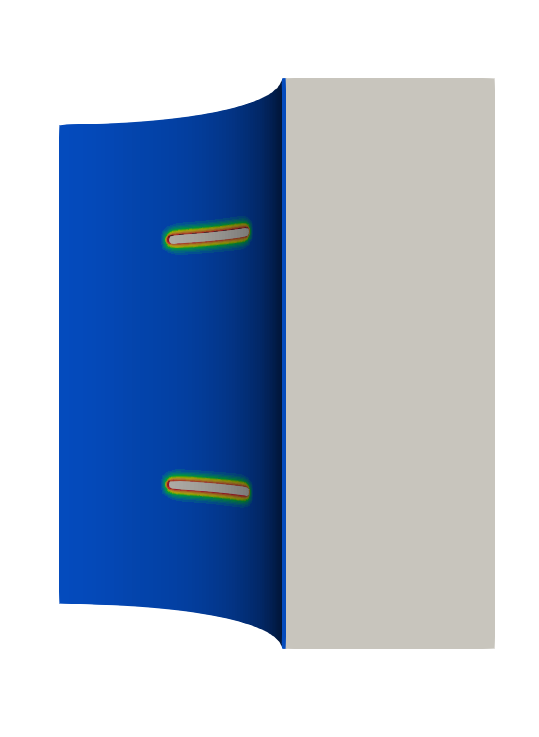
\includegraphics[width=0.7\textwidth]{examples/figures/seed_d_1}
          \end{subfigure}
        }
        
        \only<8->{
          \begin{subfigure}{0.25\textwidth}
            \centering
            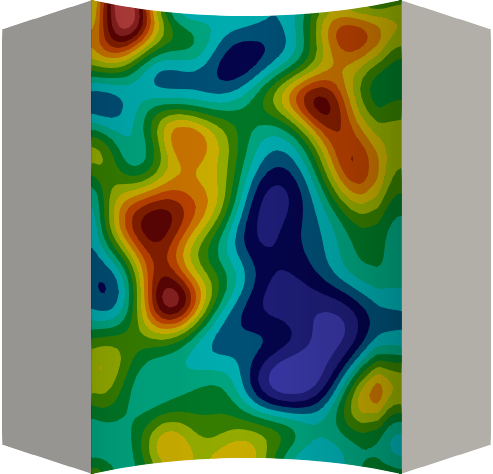
\includegraphics[width=\textwidth]{examples/figures/E.0000}
          \end{subfigure}
          \begin{subfigure}{0.1\textwidth}
            \centering
            \caption*{$E/\underline{E}$}
            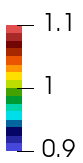
\includegraphics[width=\textwidth]{examples/figures/colorbar_rf}
          \end{subfigure}
          \hspace{0.1\textwidth}
          \begin{subfigure}{0.25\textwidth}
            \centering
            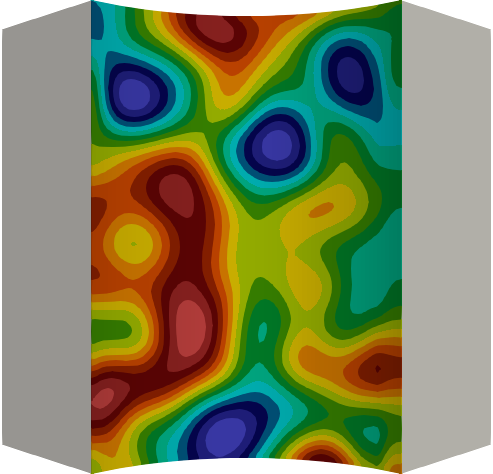
\includegraphics[width=\textwidth]{examples/figures/Gc.0000}
          \end{subfigure}
          \begin{subfigure}{0.1\textwidth}
            \centering
            \caption*{$\Gc/\underline{\Gc}$}
            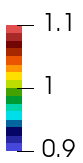
\includegraphics[width=\textwidth]{examples/figures/colorbar_rf}
          \end{subfigure}
        }
        
        \only<1-7>{
          \begin{subfigure}{\textwidth}
            \caption*{Case I: Initial transverse cracks}
          \end{subfigure}
          
          \vspace{-1em}
          
          \begin{subfigure}{0.15\textwidth}
            \caption*{}
          \end{subfigure}
          \begin{subfigure}{0.19\textwidth}
            \centering
            \caption*{$c$}
          \end{subfigure}
          \hspace{0.06\textwidth}
          \begin{subfigure}{0.19\textwidth}
            \centering
            \caption*{$d$}
          \end{subfigure}
          \hspace{0.06\textwidth}
          \begin{subfigure}{0.19\textwidth}
            \centering
            \caption*{$\ep$}
          \end{subfigure}
          
          \vspace{-1em}
          
          \begin{subfigure}{0.15\textwidth}
            \caption*{}
          \end{subfigure}
          \begin{subfigure}{0.19\textwidth}
            \centering
            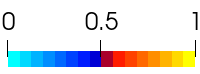
\includegraphics[width=\textwidth]{examples/figures/colorbar_c_rf}
          \end{subfigure}
          \hspace{0.06\textwidth}
          \begin{subfigure}{0.19\textwidth}
            \centering
            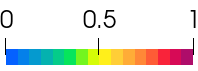
\includegraphics[width=\textwidth]{examples/figures/colorbar_d_rf}
          \end{subfigure}
          \hspace{0.06\textwidth}
          \begin{subfigure}{0.19\textwidth}
            \centering
            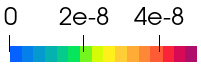
\includegraphics[width=\textwidth]{examples/figures/colorbar_ep_rf}
          \end{subfigure}
        }
        
        \only<1>{
          \begin{subfigure}{0.15\textwidth}
            \centering
            \caption*{0 day}
          \end{subfigure}
          \begin{subfigure}{0.19\textwidth}
            \centering
            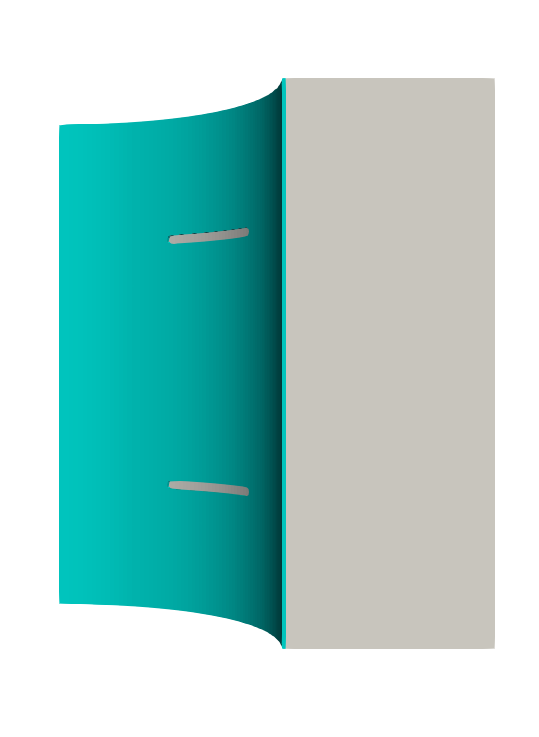
\includegraphics[width=\textwidth]{examples/figures/seed_c_1}
          \end{subfigure}
          \hspace{0.06\textwidth}
          \begin{subfigure}{0.19\textwidth}
            \centering
            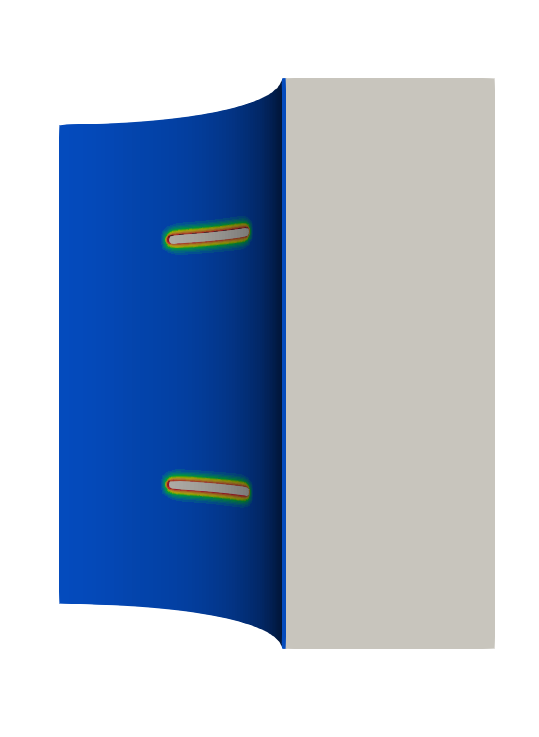
\includegraphics[width=\textwidth]{examples/figures/seed_d_1}
          \end{subfigure}
          \hspace{0.06\textwidth}
          \begin{subfigure}{0.19\textwidth}
            \centering
            
\includegraphics[width=\textwidth]{examples/figures/seed_ep_1}
          \end{subfigure}
        }
        
        \only<2>{
          \begin{subfigure}{0.15\textwidth}
            \centering
            \caption*{60 days}
          \end{subfigure}
          \begin{subfigure}{0.19\textwidth}
            \centering
            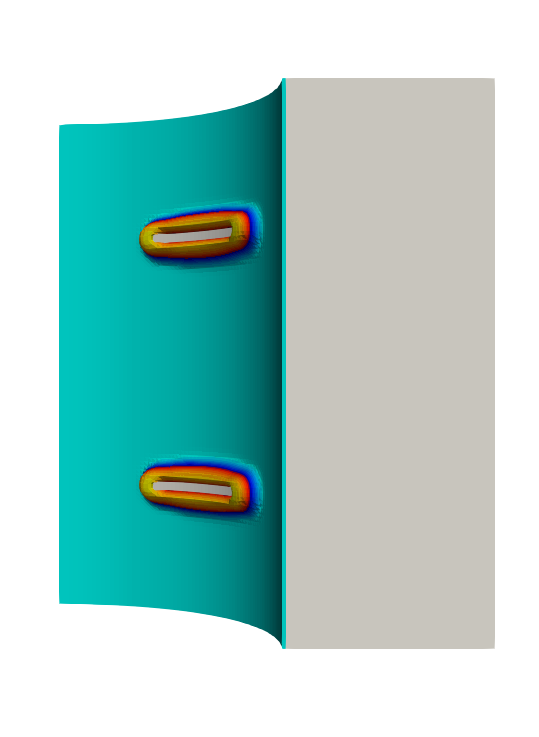
\includegraphics[width=\textwidth]{examples/figures/seed_c_2}
          \end{subfigure}
          \hspace{0.06\textwidth}
          \begin{subfigure}{0.19\textwidth}
            \centering
            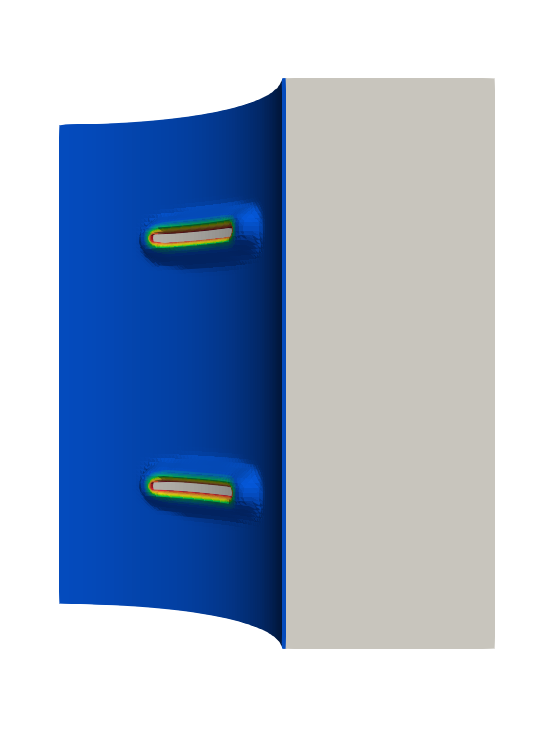
\includegraphics[width=\textwidth]{examples/figures/seed_d_2}
          \end{subfigure}
          \hspace{0.06\textwidth}
          \begin{subfigure}{0.19\textwidth}
            \centering
            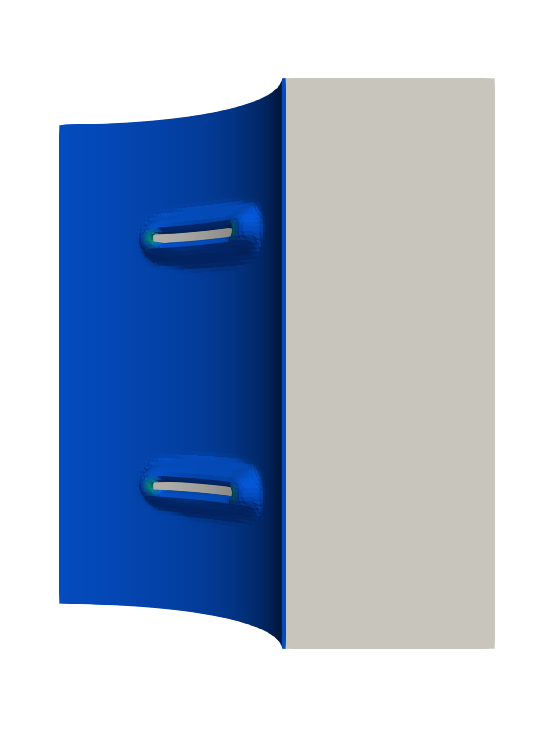
\includegraphics[width=\textwidth]{examples/figures/seed_ep_2}
          \end{subfigure}
        }
        
        \only<3>{
          \begin{subfigure}{0.15\textwidth}
            \centering
            \caption*{120 days}
          \end{subfigure}
          \begin{subfigure}{0.19\textwidth}
            \centering
            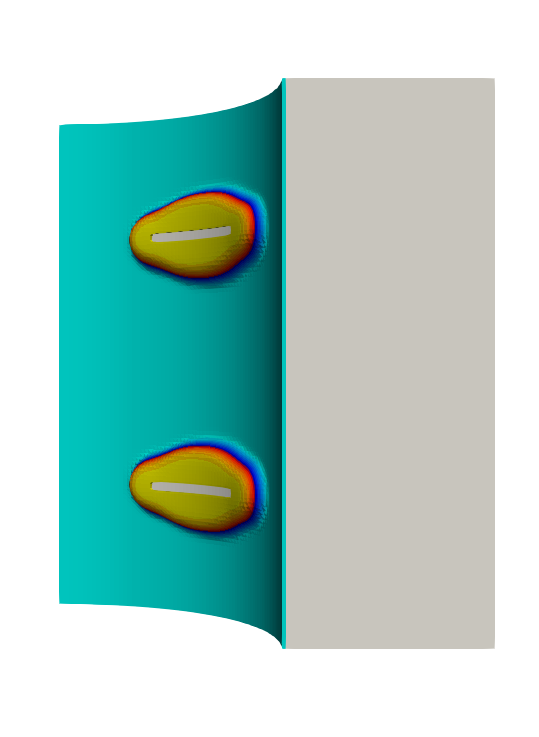
\includegraphics[width=\textwidth]{examples/figures/seed_c_3}
          \end{subfigure}
          \hspace{0.06\textwidth}
          \begin{subfigure}{0.19\textwidth}
            \centering
            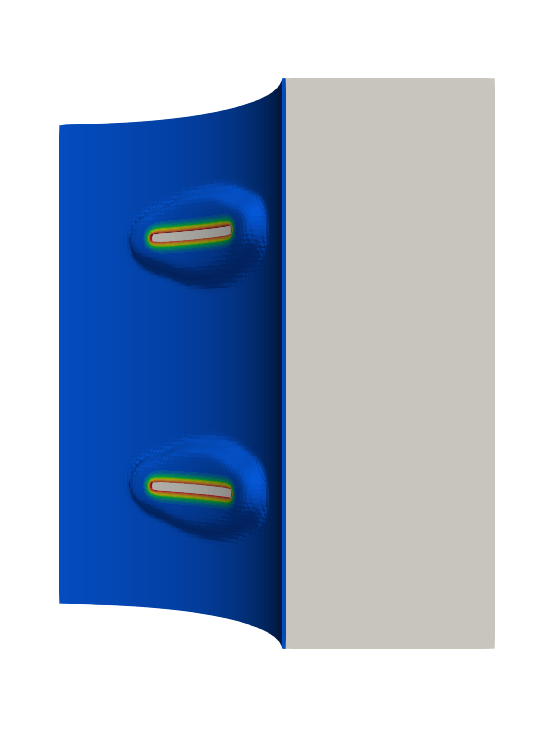
\includegraphics[width=\textwidth]{examples/figures/seed_d_3}
          \end{subfigure}
          \hspace{0.06\textwidth}
          \begin{subfigure}{0.19\textwidth}
            \centering
            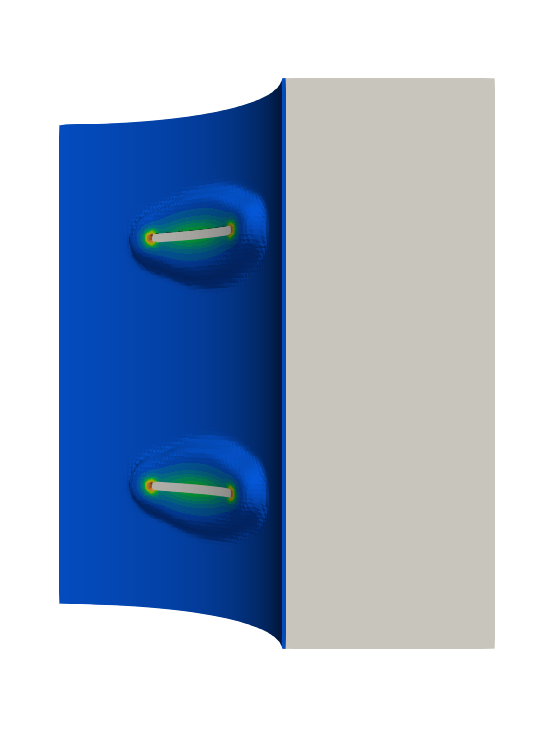
\includegraphics[width=\textwidth]{examples/figures/seed_ep_3}
          \end{subfigure}
        }
        
        \only<4>{
          \begin{subfigure}{0.15\textwidth}
            \centering
            \caption*{180 days}
          \end{subfigure}
          \begin{subfigure}{0.19\textwidth}
            \centering
            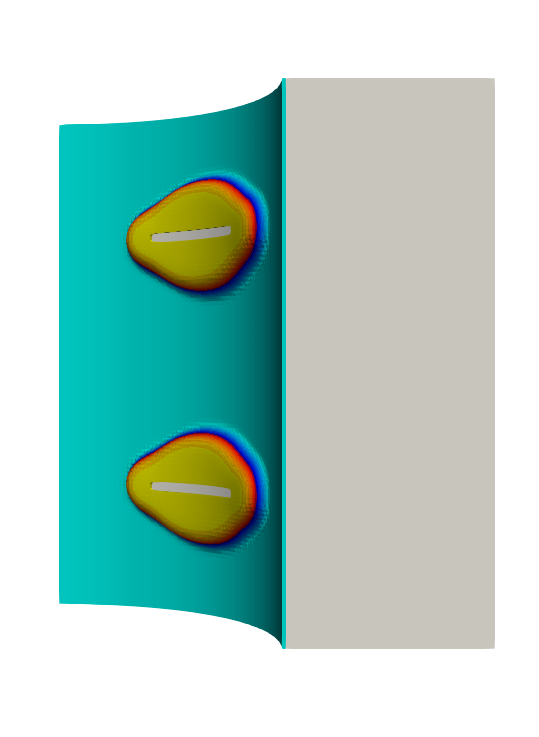
\includegraphics[width=\textwidth]{examples/figures/seed_c_4}
          \end{subfigure}
          \hspace{0.06\textwidth}
          \begin{subfigure}{0.19\textwidth}
            \centering
            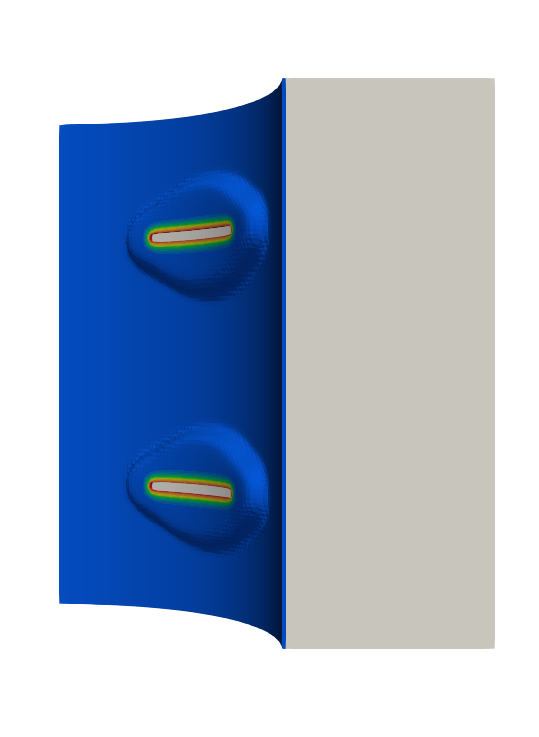
\includegraphics[width=\textwidth]{examples/figures/seed_d_4}
          \end{subfigure}
          \hspace{0.06\textwidth}
          \begin{subfigure}{0.19\textwidth}
            \centering
            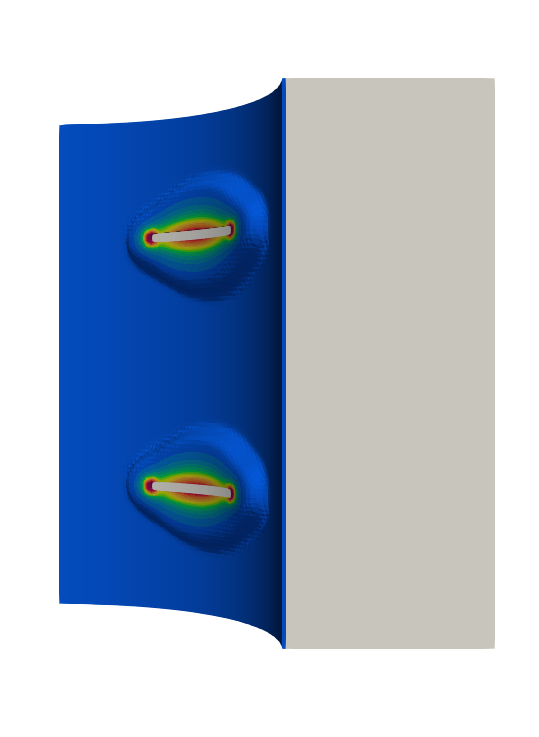
\includegraphics[width=\textwidth]{examples/figures/seed_ep_4}
          \end{subfigure}
        }
        
        \only<5>{
          \begin{subfigure}{0.15\textwidth}
            \centering
            \caption*{1 hour}
          \end{subfigure}
          \begin{subfigure}{0.19\textwidth}
            \centering
            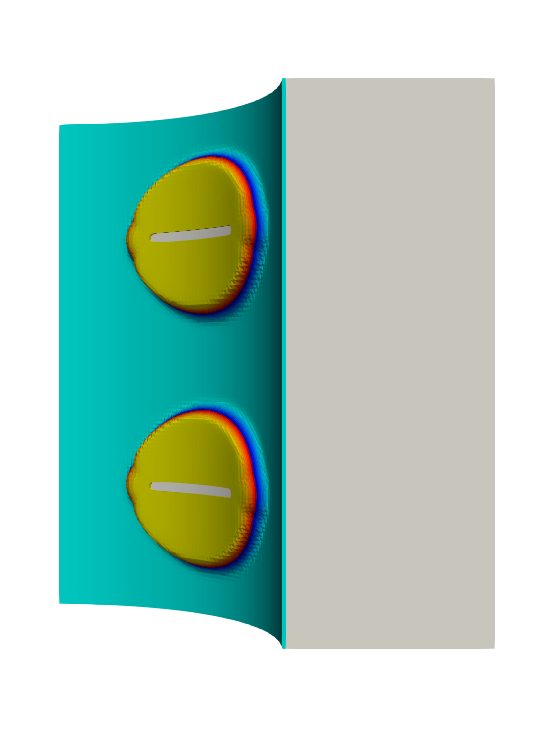
\includegraphics[width=\textwidth]{examples/figures/seed_c_5}
          \end{subfigure}
          \hspace{0.06\textwidth}
          \begin{subfigure}{0.19\textwidth}
            \centering
            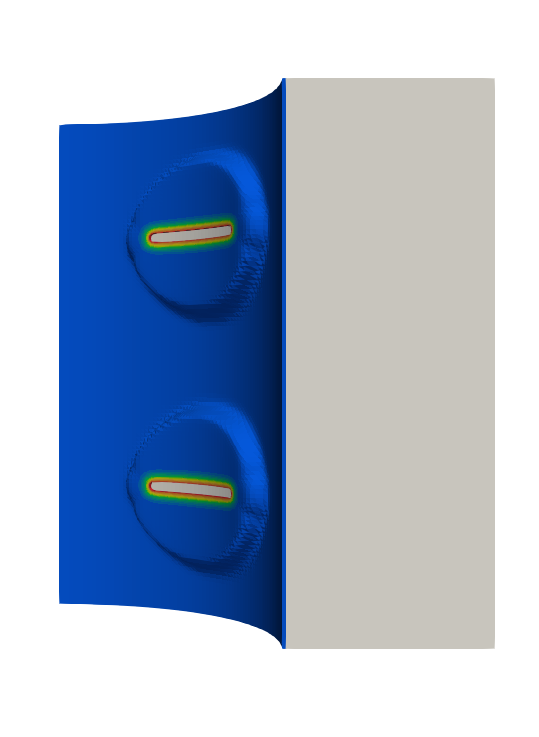
\includegraphics[width=\textwidth]{examples/figures/seed_d_5}
          \end{subfigure}
          \hspace{0.06\textwidth}
          \begin{subfigure}{0.19\textwidth}
            \centering
            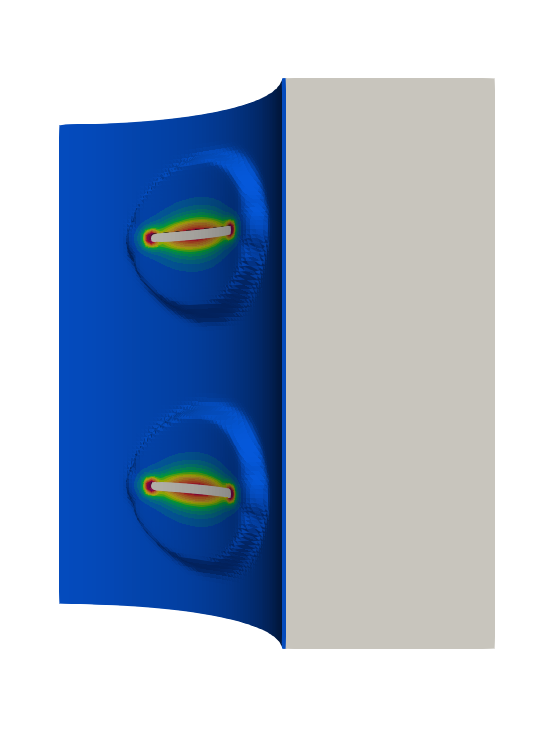
\includegraphics[width=\textwidth]{examples/figures/seed_ep_5}
          \end{subfigure}
        }
        
        \only<6>{
          \begin{subfigure}{0.15\textwidth}
            \centering
            \caption*{2 hours}
          \end{subfigure}
          \begin{subfigure}{0.19\textwidth}
            \centering
            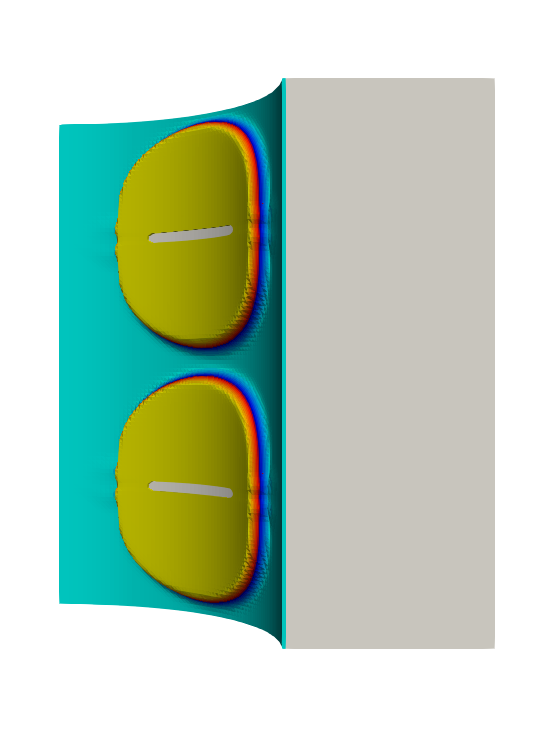
\includegraphics[width=\textwidth]{examples/figures/seed_c_6}
          \end{subfigure}
          \hspace{0.06\textwidth}
          \begin{subfigure}{0.19\textwidth}
            \centering
            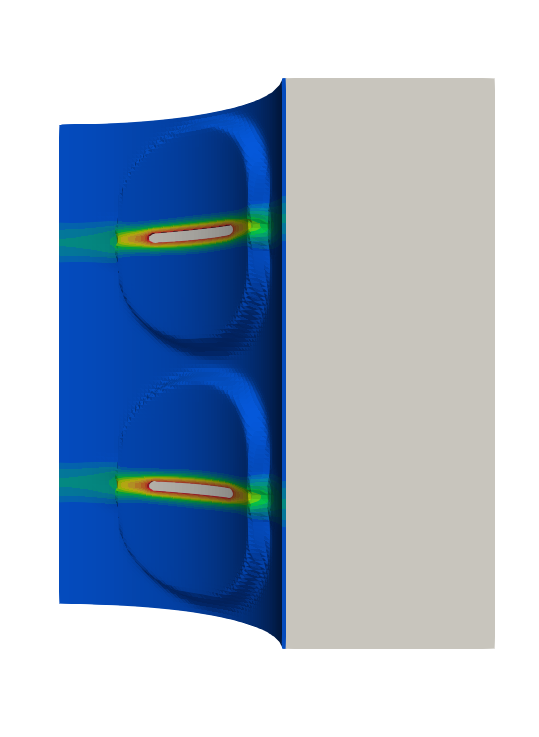
\includegraphics[width=\textwidth]{examples/figures/seed_d_6}
          \end{subfigure}
          \hspace{0.06\textwidth}
          \begin{subfigure}{0.19\textwidth}
            \centering
            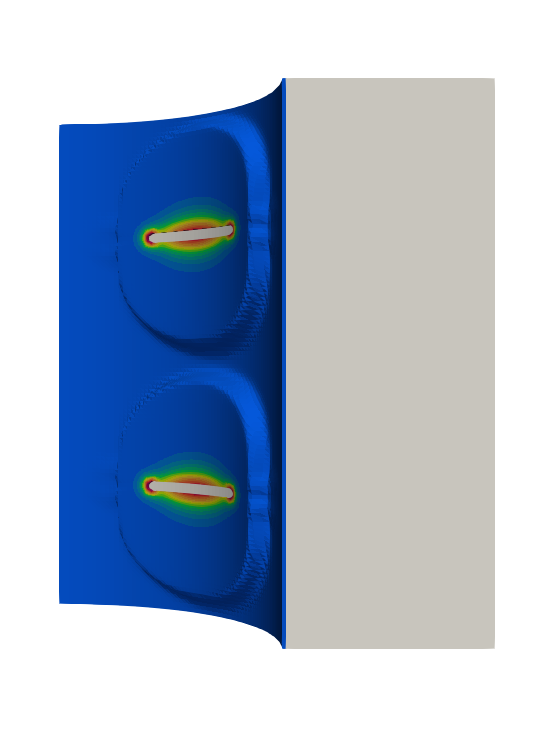
\includegraphics[width=\textwidth]{examples/figures/seed_ep_6}
          \end{subfigure}
        }
        
        \only<7>{
          \begin{subfigure}{0.15\textwidth}
            \centering
            \caption*{3 hours}
          \end{subfigure}
          \begin{subfigure}{0.19\textwidth}
            \centering
            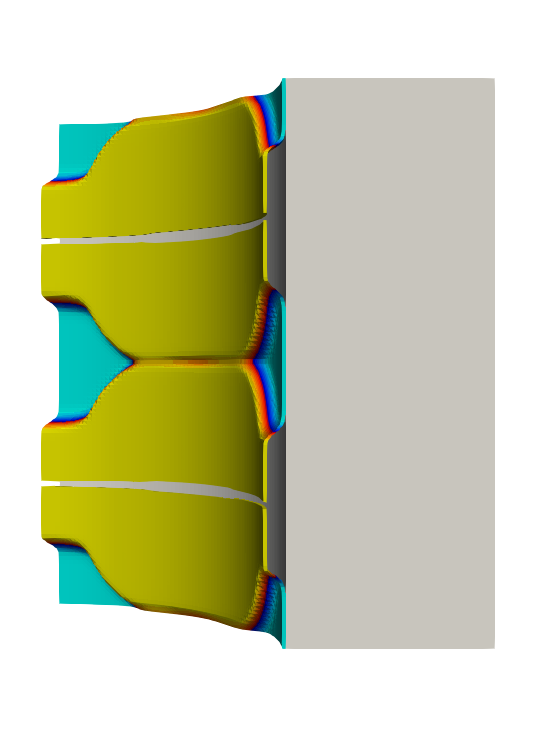
\includegraphics[width=\textwidth]{examples/figures/seed_c_7}
          \end{subfigure}
          \hspace{0.06\textwidth}
          \begin{subfigure}{0.19\textwidth}
            \centering
            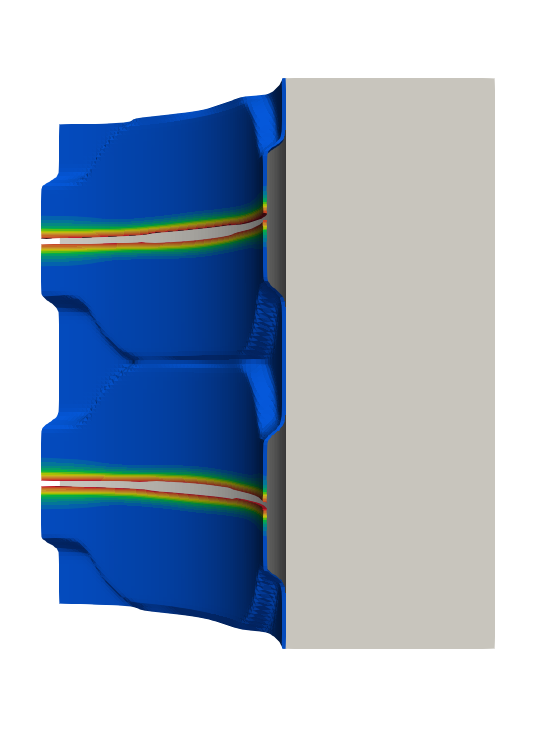
\includegraphics[width=\textwidth]{examples/figures/seed_d_7}
          \end{subfigure}
          \hspace{0.06\textwidth}
          \begin{subfigure}{0.19\textwidth}
            \centering
            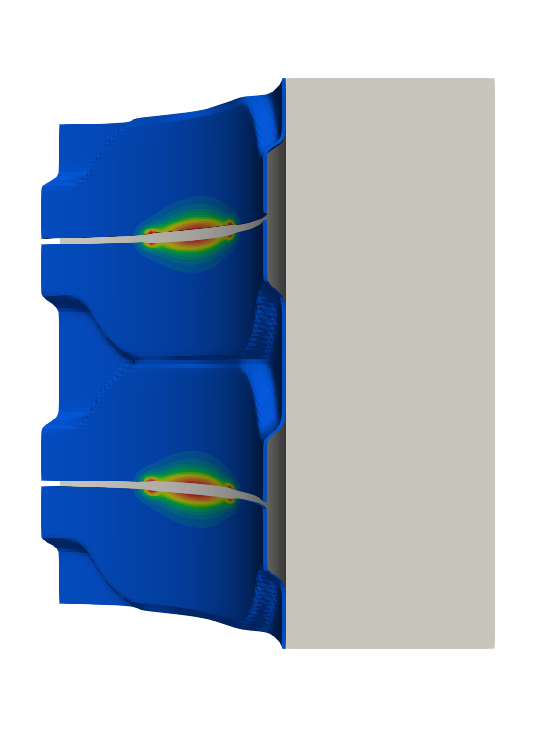
\includegraphics[width=\textwidth]{examples/figures/seed_ep_7}
          \end{subfigure}
        }
        
        \only<9->{
          \begin{subfigure}{\textwidth}
            \caption*{Case II: Inhomogeneous Young's modulus and Fracture toughness}
          \end{subfigure}
          
          \vspace{-1em}
          
          \begin{subfigure}{0.15\textwidth}
            \caption*{}
          \end{subfigure}
          \begin{subfigure}{0.19\textwidth}
            \centering
            \caption*{$c$}
          \end{subfigure}
          \hspace{0.06\textwidth}
          \begin{subfigure}{0.19\textwidth}
            \centering
            \caption*{$d$}
          \end{subfigure}
          \hspace{0.06\textwidth}
          \begin{subfigure}{0.19\textwidth}
            \centering
            \caption*{$\ep$}
          \end{subfigure}
          
          \vspace{-1em}
          
          \begin{subfigure}{0.15\textwidth}
            \caption*{}
          \end{subfigure}
          \begin{subfigure}{0.19\textwidth}
            \centering
            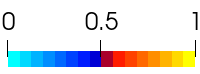
\includegraphics[width=\textwidth]{examples/figures/colorbar_c_rf}
          \end{subfigure}
          \hspace{0.06\textwidth}
          \begin{subfigure}{0.19\textwidth}
            \centering
            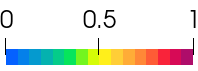
\includegraphics[width=\textwidth]{examples/figures/colorbar_d_rf}
          \end{subfigure}
          \hspace{0.06\textwidth}
          \begin{subfigure}{0.19\textwidth}
            \centering
            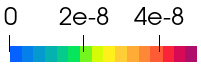
\includegraphics[width=\textwidth]{examples/figures/colorbar_ep_rf}
          \end{subfigure}
        }
        
        \only<9>{
          \begin{subfigure}{0.15\textwidth}
            \centering
            \caption*{30 days}
          \end{subfigure}
          \begin{subfigure}{0.19\textwidth}
            \centering
            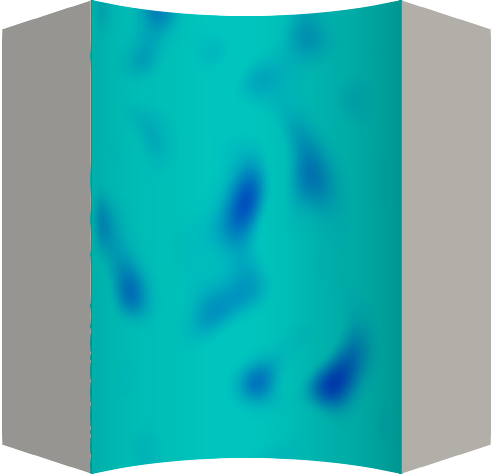
\includegraphics[width=\textwidth]{examples/figures/c.0003}
          \end{subfigure}
          \hspace{0.06\textwidth}
          \begin{subfigure}{0.19\textwidth}
            \centering
            \includegraphics[width=\textwidth]{examples/figures/d.0003}
          \end{subfigure}
          \hspace{0.06\textwidth}
          \begin{subfigure}{0.19\textwidth}
            \centering
            \includegraphics[width=\textwidth]{examples/figures/ep.0003}
          \end{subfigure}
        }
        
        \only<10>{
          \begin{subfigure}{0.15\textwidth}
            \centering
            \caption*{60 days}
          \end{subfigure}
          \begin{subfigure}{0.19\textwidth}
            \centering
            \includegraphics[width=\textwidth]{examples/figures/c.0006}
          \end{subfigure}
          \hspace{0.06\textwidth}
          \begin{subfigure}{0.19\textwidth}
            \centering
            \includegraphics[width=\textwidth]{examples/figures/d.0006}
          \end{subfigure}
          \hspace{0.06\textwidth}
          \begin{subfigure}{0.19\textwidth}
            \centering
            \includegraphics[width=\textwidth]{examples/figures/ep.0006}
          \end{subfigure}
        }
        
        \only<11>{
          \begin{subfigure}{0.15\textwidth}
            \centering
            \caption*{90 days}
          \end{subfigure}
          \begin{subfigure}{0.19\textwidth}
            \centering
            \includegraphics[width=\textwidth]{examples/figures/c.0009}
          \end{subfigure}
          \hspace{0.06\textwidth}
          \begin{subfigure}{0.19\textwidth}
            \centering
            \includegraphics[width=\textwidth]{examples/figures/d.0009}
          \end{subfigure}
          \hspace{0.06\textwidth}
          \begin{subfigure}{0.19\textwidth}
            \centering
            \includegraphics[width=\textwidth]{examples/figures/ep.0009}
          \end{subfigure}
        }
        
        \only<12>{
          \begin{subfigure}{0.15\textwidth}
            \centering
            \caption*{120 days}
          \end{subfigure}
          \begin{subfigure}{0.19\textwidth}
            \centering
            \includegraphics[width=\textwidth]{examples/figures/c.0012}
          \end{subfigure}
          \hspace{0.06\textwidth}
          \begin{subfigure}{0.19\textwidth}
            \centering
            \includegraphics[width=\textwidth]{examples/figures/d.0012}
          \end{subfigure}
          \hspace{0.06\textwidth}
          \begin{subfigure}{0.19\textwidth}
            \centering
            \includegraphics[width=\textwidth]{examples/figures/ep.0012}
          \end{subfigure}
        }
        
        \only<13>{
          \begin{subfigure}{0.15\textwidth}
            \centering
            \caption*{150 days}
          \end{subfigure}
          \begin{subfigure}{0.19\textwidth}
            \centering
            \includegraphics[width=\textwidth]{examples/figures/c.0015}
          \end{subfigure}
          \hspace{0.06\textwidth}
          \begin{subfigure}{0.19\textwidth}
            \centering
            \includegraphics[width=\textwidth]{examples/figures/d.0015}
          \end{subfigure}
          \hspace{0.06\textwidth}
          \begin{subfigure}{0.19\textwidth}
            \centering
            \includegraphics[width=\textwidth]{examples/figures/ep.0015}
          \end{subfigure}
        }
        
        \only<14>{
          \begin{subfigure}{0.15\textwidth}
            \centering
            \caption*{180 days}
          \end{subfigure}
          \begin{subfigure}{0.19\textwidth}
            \centering
            \includegraphics[width=\textwidth]{examples/figures/c.0018}
          \end{subfigure}
          \hspace{0.06\textwidth}
          \begin{subfigure}{0.19\textwidth}
            \centering
            \includegraphics[width=\textwidth]{examples/figures/d.0018}
          \end{subfigure}
          \hspace{0.06\textwidth}
          \begin{subfigure}{0.19\textwidth}
            \centering
            \includegraphics[width=\textwidth]{examples/figures/ep.0018}
          \end{subfigure}
        }
        
        \only<15>{
          \begin{subfigure}{0.15\textwidth}
            \centering
            \caption*{1 hour}
          \end{subfigure}
          \begin{subfigure}{0.19\textwidth}
            \centering
            \includegraphics[width=\textwidth]{examples/figures/c.0021}
          \end{subfigure}
          \hspace{0.06\textwidth}
          \begin{subfigure}{0.19\textwidth}
            \centering
            \includegraphics[width=\textwidth]{examples/figures/d.0021}
          \end{subfigure}
          \hspace{0.06\textwidth}
          \begin{subfigure}{0.19\textwidth}
            \centering
            \includegraphics[width=\textwidth]{examples/figures/ep.0021}
          \end{subfigure}
        }
        
        \only<16>{
          \begin{subfigure}{0.15\textwidth}
            \centering
            \caption*{2 hours}
          \end{subfigure}
          \begin{subfigure}{0.19\textwidth}
            \centering
            \includegraphics[width=\textwidth]{examples/figures/c.0024}
          \end{subfigure}
          \hspace{0.06\textwidth}
          \begin{subfigure}{0.19\textwidth}
            \centering
            \includegraphics[width=\textwidth]{examples/figures/d.0024}
          \end{subfigure}
          \hspace{0.06\textwidth}
          \begin{subfigure}{0.19\textwidth}
            \centering
            \includegraphics[width=\textwidth]{examples/figures/ep.0024}
          \end{subfigure}
        }
        
        \only<17>{
          \begin{subfigure}{0.15\textwidth}
            \centering
            \caption*{3 hours}
          \end{subfigure}
          \begin{subfigure}{0.19\textwidth}
            \centering
            \includegraphics[width=\textwidth]{examples/figures/c.0027}
          \end{subfigure}
          \hspace{0.06\textwidth}
          \begin{subfigure}{0.19\textwidth}
            \centering
            \includegraphics[width=\textwidth]{examples/figures/d.0027}
          \end{subfigure}
          \hspace{0.06\textwidth}
          \begin{subfigure}{0.19\textwidth}
            \centering
            \includegraphics[width=\textwidth]{examples/figures/ep.0027}
          \end{subfigure}
        }
        
        \only<18>{
          \begin{subfigure}{0.15\textwidth}
            \centering
            \caption*{4 hours}
          \end{subfigure}
          \begin{subfigure}{0.19\textwidth}
            \centering
            \includegraphics[width=\textwidth]{examples/figures/c.0030}
          \end{subfigure}
          \hspace{0.06\textwidth}
          \begin{subfigure}{0.19\textwidth}
            \centering
            \includegraphics[width=\textwidth]{examples/figures/d.0030}
          \end{subfigure}
          \hspace{0.06\textwidth}
          \begin{subfigure}{0.19\textwidth}
            \centering
            \includegraphics[width=\textwidth]{examples/figures/ep.0030}
          \end{subfigure}
        }
        
        \only<19>{
          \begin{subfigure}{0.15\textwidth}
            \centering
            \caption*{5 hours}
          \end{subfigure}
          \begin{subfigure}{0.19\textwidth}
            \centering
            \includegraphics[width=\textwidth]{examples/figures/c.0033}
          \end{subfigure}
          \hspace{0.06\textwidth}
          \begin{subfigure}{0.19\textwidth}
            \centering
            \includegraphics[width=\textwidth]{examples/figures/d.0033}
          \end{subfigure}
          \hspace{0.06\textwidth}
          \begin{subfigure}{0.19\textwidth}
            \centering
            \includegraphics[width=\textwidth]{examples/figures/ep.0033}
          \end{subfigure}
        }
        
        \only<20>{
          \begin{subfigure}{0.15\textwidth}
            \centering
            \caption*{6 hours}
          \end{subfigure}
          \begin{subfigure}{0.19\textwidth}
            \centering
            \includegraphics[width=\textwidth]{examples/figures/c.0036}
          \end{subfigure}
          \hspace{0.06\textwidth}
          \begin{subfigure}{0.19\textwidth}
            \centering
            \includegraphics[width=\textwidth]{examples/figures/d.0036}
          \end{subfigure}
          \hspace{0.06\textwidth}
          \begin{subfigure}{0.19\textwidth}
            \centering
            \includegraphics[width=\textwidth]{examples/figures/ep.0036}
          \end{subfigure}
        }
      \end{figure}
    \end{column}
    \begin{column}{0.4\textwidth}
      \begin{itemize}
        \item The HTHX is simulated for 180 days under \textcolor{peggyblue}{normal operating conditions}, followed by a \textcolor{peggyblue}{shutdown} (6-hour transition).
        \item The HTHX is surround by \textcolor{peggyblue}{high temperature pressurized} fluids during normal operation. The temperature and the pressure of the fluids drop after shutting down.
        \item Most model parameters are adopted from \cite{xue2020stress}.
        \item[\textcolor{peggyblue}{\textbullet}] Creep deformation accumulates under normal operating conditions. The effective creep strain localizes around the cracks.
        \item[\textcolor{peggyblue}{\textbullet}] Debonding occurs at weaker locations in the vicinity of the crack surfaces.
        \item[\textcolor{peggyblue}{\textbullet}] Transverse cracks nucleate and propagate while shutting down.
      \end{itemize}
    \end{column}
  \end{columns}
\end{frame}
